% PRIME Architecture Diagram (TikZ)
% Include this in main.tex with: % PRIME Architecture Diagram (TikZ)
% Include this in main.tex with: % PRIME Architecture Diagram (TikZ)
% Include this in main.tex with: % PRIME Architecture Diagram (TikZ)
% Include this in main.tex with: \input{figures/architecture.tex}

\begin{figure*}[t]
\centering
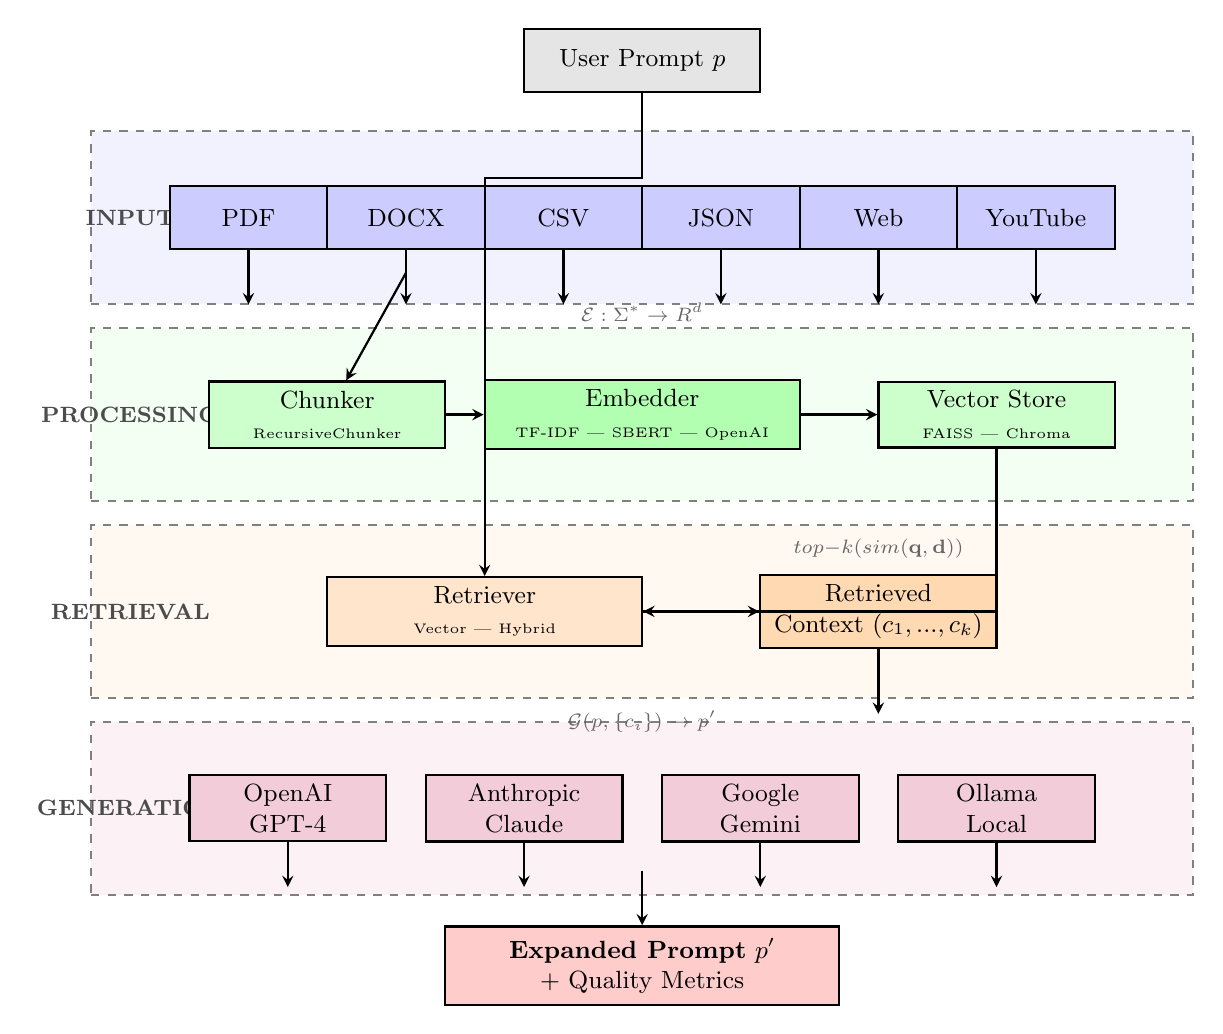
\begin{tikzpicture}[
    node distance=0.8cm and 1.2cm,
    box/.style={rectangle, draw=black, thick, minimum width=2cm, minimum height=0.8cm, align=center, font=\small},
    layer/.style={rectangle, draw=black!50, dashed, thick, minimum width=14cm, minimum height=2.2cm, align=center},
    arrow/.style={->, thick, >=stealth},
    label/.style={font=\footnotesize\bfseries, text=black!70}
]

% Layer backgrounds
\node[layer, fill=blue!5] (input_layer) at (0, 6) {};
\node[layer, fill=green!5] (process_layer) at (0, 3.5) {};
\node[layer, fill=orange!5] (retrieval_layer) at (0, 1) {};
\node[layer, fill=purple!5] (generation_layer) at (0, -1.5) {};

% Layer labels
\node[label] at (-6.5, 6) {INPUT};
\node[label] at (-6.5, 3.5) {PROCESSING};
\node[label] at (-6.5, 1) {RETRIEVAL};
\node[label] at (-6.5, -1.5) {GENERATION};

% Input Layer - Document Loaders
\node[box, fill=blue!20] (pdf) at (-5, 6) {PDF};
\node[box, fill=blue!20] (docx) at (-3, 6) {DOCX};
\node[box, fill=blue!20] (csv) at (-1, 6) {CSV};
\node[box, fill=blue!20] (json) at (1, 6) {JSON};
\node[box, fill=blue!20] (web) at (3, 6) {Web};
\node[box, fill=blue!20] (youtube) at (5, 6) {YouTube};

% Processing Layer
\node[box, fill=green!20, minimum width=3cm] (chunker) at (-4, 3.5) {Chunker\\{\tiny RecursiveChunker}};
\node[box, fill=green!30, minimum width=4cm] (embedder) at (0, 3.5) {Embedder\\{\tiny TF-IDF | SBERT | OpenAI}};
\node[box, fill=green!20, minimum width=3cm] (vectorstore) at (4.5, 3.5) {Vector Store\\{\tiny FAISS | Chroma}};

% Retrieval Layer
\node[box, fill=orange!20, minimum width=4cm] (retriever) at (-2, 1) {Retriever\\{\tiny Vector | Hybrid}};
\node[box, fill=orange!30, minimum width=3cm] (context) at (3, 1) {Retrieved\\Context $(c_1,...,c_k)$};

% Generation Layer
\node[box, fill=purple!20, minimum width=2.5cm] (openai) at (-4.5, -1.5) {OpenAI\\GPT-4};
\node[box, fill=purple!20, minimum width=2.5cm] (anthropic) at (-1.5, -1.5) {Anthropic\\Claude};
\node[box, fill=purple!20, minimum width=2.5cm] (google) at (1.5, -1.5) {Google\\Gemini};
\node[box, fill=purple!20, minimum width=2.5cm] (ollama) at (4.5, -1.5) {Ollama\\Local};

% Output
\node[box, fill=red!20, minimum width=5cm, minimum height=1cm] (output) at (0, -3.5) {\textbf{Expanded Prompt} $p'$\\+ Quality Metrics};

% User Input
\node[box, fill=gray!20, minimum width=3cm] (user) at (0, 8) {User Prompt $p$};

% Arrows - Input flow
\foreach \x in {pdf, docx, csv, json, web, youtube} {
    \draw[arrow] (\x) -- +(0, -1.1);
}

% Arrows - Processing flow
\draw[arrow] (-3, 5.3) -- (chunker);
\draw[arrow] (chunker) -- (embedder);
\draw[arrow] (embedder) -- (vectorstore);

% Arrows - Retrieval flow
\draw[arrow] (user) -- +(0, -1.5) -| (retriever);
\draw[arrow] (vectorstore) |- (retriever);
\draw[arrow] (retriever) -- (context);

% Arrows - Generation flow
\draw[arrow] (context) -- +(0, -1.3);
\foreach \g in {openai, anthropic, google, ollama} {
    \draw[arrow] (\g) -- +(0, -1);
}

% Output arrow
\draw[arrow] (0, -2.3) -- (output);

% Formulas
\node[font=\scriptsize, text=black!60] at (0, 4.8) {$\mathcal{E}: \Sigma^* \rightarrow \mathbb{R}^d$};
\node[font=\scriptsize, text=black!60] at (3, 1.8) {$\text{top-}k(\text{sim}(\mathbf{q}, \mathbf{d}))$};
\node[font=\scriptsize, text=black!60] at (0, -0.4) {$\mathcal{G}(p, \{c_i\}) \rightarrow p'$};

\end{tikzpicture}
\caption{PRIME system architecture showing the five-layer pipeline: Input (document loaders), Processing (chunking and embedding), Storage (vector stores), Retrieval (similarity search), and Generation (LLM-based prompt expansion). Each layer implements pluggable components via abstract interfaces.}
\label{fig:architecture}
\end{figure*}



\begin{figure*}[t]
\centering
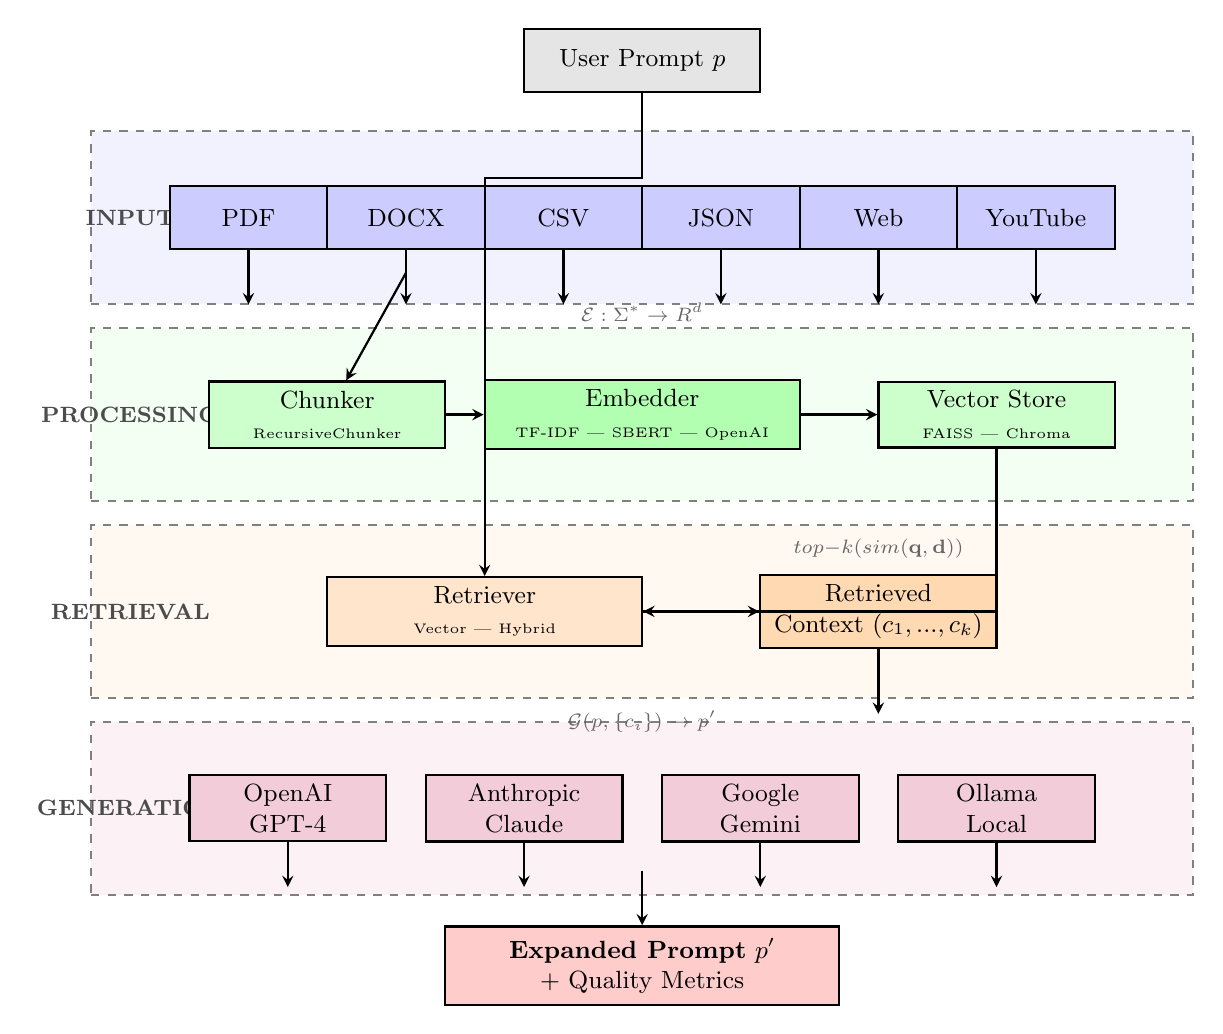
\begin{tikzpicture}[
    node distance=0.8cm and 1.2cm,
    box/.style={rectangle, draw=black, thick, minimum width=2cm, minimum height=0.8cm, align=center, font=\small},
    layer/.style={rectangle, draw=black!50, dashed, thick, minimum width=14cm, minimum height=2.2cm, align=center},
    arrow/.style={->, thick, >=stealth},
    label/.style={font=\footnotesize\bfseries, text=black!70}
]

% Layer backgrounds
\node[layer, fill=blue!5] (input_layer) at (0, 6) {};
\node[layer, fill=green!5] (process_layer) at (0, 3.5) {};
\node[layer, fill=orange!5] (retrieval_layer) at (0, 1) {};
\node[layer, fill=purple!5] (generation_layer) at (0, -1.5) {};

% Layer labels
\node[label] at (-6.5, 6) {INPUT};
\node[label] at (-6.5, 3.5) {PROCESSING};
\node[label] at (-6.5, 1) {RETRIEVAL};
\node[label] at (-6.5, -1.5) {GENERATION};

% Input Layer - Document Loaders
\node[box, fill=blue!20] (pdf) at (-5, 6) {PDF};
\node[box, fill=blue!20] (docx) at (-3, 6) {DOCX};
\node[box, fill=blue!20] (csv) at (-1, 6) {CSV};
\node[box, fill=blue!20] (json) at (1, 6) {JSON};
\node[box, fill=blue!20] (web) at (3, 6) {Web};
\node[box, fill=blue!20] (youtube) at (5, 6) {YouTube};

% Processing Layer
\node[box, fill=green!20, minimum width=3cm] (chunker) at (-4, 3.5) {Chunker\\{\tiny RecursiveChunker}};
\node[box, fill=green!30, minimum width=4cm] (embedder) at (0, 3.5) {Embedder\\{\tiny TF-IDF | SBERT | OpenAI}};
\node[box, fill=green!20, minimum width=3cm] (vectorstore) at (4.5, 3.5) {Vector Store\\{\tiny FAISS | Chroma}};

% Retrieval Layer
\node[box, fill=orange!20, minimum width=4cm] (retriever) at (-2, 1) {Retriever\\{\tiny Vector | Hybrid}};
\node[box, fill=orange!30, minimum width=3cm] (context) at (3, 1) {Retrieved\\Context $(c_1,...,c_k)$};

% Generation Layer
\node[box, fill=purple!20, minimum width=2.5cm] (openai) at (-4.5, -1.5) {OpenAI\\GPT-4};
\node[box, fill=purple!20, minimum width=2.5cm] (anthropic) at (-1.5, -1.5) {Anthropic\\Claude};
\node[box, fill=purple!20, minimum width=2.5cm] (google) at (1.5, -1.5) {Google\\Gemini};
\node[box, fill=purple!20, minimum width=2.5cm] (ollama) at (4.5, -1.5) {Ollama\\Local};

% Output
\node[box, fill=red!20, minimum width=5cm, minimum height=1cm] (output) at (0, -3.5) {\textbf{Expanded Prompt} $p'$\\+ Quality Metrics};

% User Input
\node[box, fill=gray!20, minimum width=3cm] (user) at (0, 8) {User Prompt $p$};

% Arrows - Input flow
\foreach \x in {pdf, docx, csv, json, web, youtube} {
    \draw[arrow] (\x) -- +(0, -1.1);
}

% Arrows - Processing flow
\draw[arrow] (-3, 5.3) -- (chunker);
\draw[arrow] (chunker) -- (embedder);
\draw[arrow] (embedder) -- (vectorstore);

% Arrows - Retrieval flow
\draw[arrow] (user) -- +(0, -1.5) -| (retriever);
\draw[arrow] (vectorstore) |- (retriever);
\draw[arrow] (retriever) -- (context);

% Arrows - Generation flow
\draw[arrow] (context) -- +(0, -1.3);
\foreach \g in {openai, anthropic, google, ollama} {
    \draw[arrow] (\g) -- +(0, -1);
}

% Output arrow
\draw[arrow] (0, -2.3) -- (output);

% Formulas
\node[font=\scriptsize, text=black!60] at (0, 4.8) {$\mathcal{E}: \Sigma^* \rightarrow \mathbb{R}^d$};
\node[font=\scriptsize, text=black!60] at (3, 1.8) {$\text{top-}k(\text{sim}(\mathbf{q}, \mathbf{d}))$};
\node[font=\scriptsize, text=black!60] at (0, -0.4) {$\mathcal{G}(p, \{c_i\}) \rightarrow p'$};

\end{tikzpicture}
\caption{PRIME system architecture showing the five-layer pipeline: Input (document loaders), Processing (chunking and embedding), Storage (vector stores), Retrieval (similarity search), and Generation (LLM-based prompt expansion). Each layer implements pluggable components via abstract interfaces.}
\label{fig:architecture}
\end{figure*}



\begin{figure*}[t]
\centering
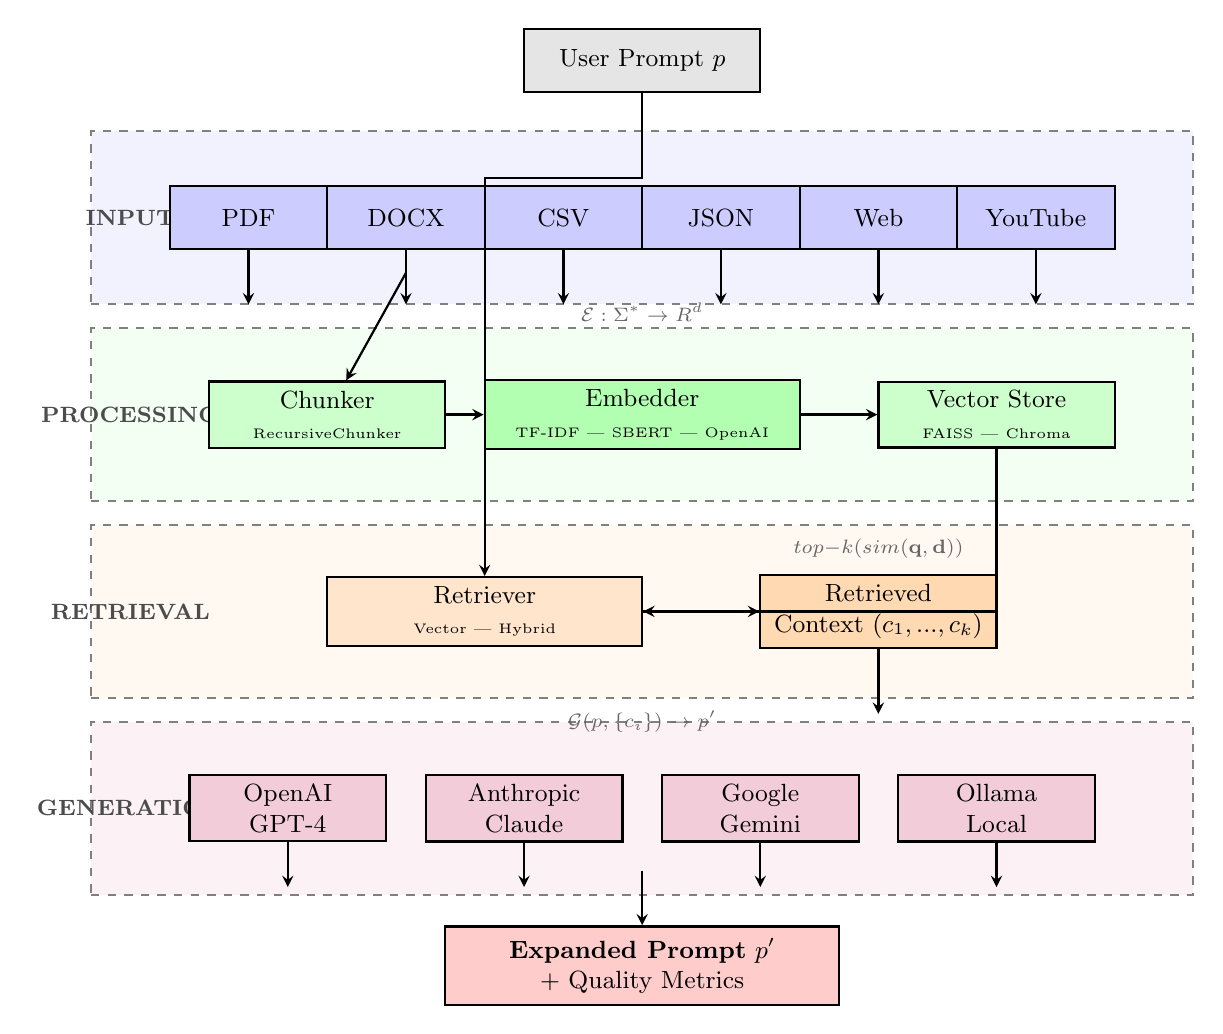
\begin{tikzpicture}[
    node distance=0.8cm and 1.2cm,
    box/.style={rectangle, draw=black, thick, minimum width=2cm, minimum height=0.8cm, align=center, font=\small},
    layer/.style={rectangle, draw=black!50, dashed, thick, minimum width=14cm, minimum height=2.2cm, align=center},
    arrow/.style={->, thick, >=stealth},
    label/.style={font=\footnotesize\bfseries, text=black!70}
]

% Layer backgrounds
\node[layer, fill=blue!5] (input_layer) at (0, 6) {};
\node[layer, fill=green!5] (process_layer) at (0, 3.5) {};
\node[layer, fill=orange!5] (retrieval_layer) at (0, 1) {};
\node[layer, fill=purple!5] (generation_layer) at (0, -1.5) {};

% Layer labels
\node[label] at (-6.5, 6) {INPUT};
\node[label] at (-6.5, 3.5) {PROCESSING};
\node[label] at (-6.5, 1) {RETRIEVAL};
\node[label] at (-6.5, -1.5) {GENERATION};

% Input Layer - Document Loaders
\node[box, fill=blue!20] (pdf) at (-5, 6) {PDF};
\node[box, fill=blue!20] (docx) at (-3, 6) {DOCX};
\node[box, fill=blue!20] (csv) at (-1, 6) {CSV};
\node[box, fill=blue!20] (json) at (1, 6) {JSON};
\node[box, fill=blue!20] (web) at (3, 6) {Web};
\node[box, fill=blue!20] (youtube) at (5, 6) {YouTube};

% Processing Layer
\node[box, fill=green!20, minimum width=3cm] (chunker) at (-4, 3.5) {Chunker\\{\tiny RecursiveChunker}};
\node[box, fill=green!30, minimum width=4cm] (embedder) at (0, 3.5) {Embedder\\{\tiny TF-IDF | SBERT | OpenAI}};
\node[box, fill=green!20, minimum width=3cm] (vectorstore) at (4.5, 3.5) {Vector Store\\{\tiny FAISS | Chroma}};

% Retrieval Layer
\node[box, fill=orange!20, minimum width=4cm] (retriever) at (-2, 1) {Retriever\\{\tiny Vector | Hybrid}};
\node[box, fill=orange!30, minimum width=3cm] (context) at (3, 1) {Retrieved\\Context $(c_1,...,c_k)$};

% Generation Layer
\node[box, fill=purple!20, minimum width=2.5cm] (openai) at (-4.5, -1.5) {OpenAI\\GPT-4};
\node[box, fill=purple!20, minimum width=2.5cm] (anthropic) at (-1.5, -1.5) {Anthropic\\Claude};
\node[box, fill=purple!20, minimum width=2.5cm] (google) at (1.5, -1.5) {Google\\Gemini};
\node[box, fill=purple!20, minimum width=2.5cm] (ollama) at (4.5, -1.5) {Ollama\\Local};

% Output
\node[box, fill=red!20, minimum width=5cm, minimum height=1cm] (output) at (0, -3.5) {\textbf{Expanded Prompt} $p'$\\+ Quality Metrics};

% User Input
\node[box, fill=gray!20, minimum width=3cm] (user) at (0, 8) {User Prompt $p$};

% Arrows - Input flow
\foreach \x in {pdf, docx, csv, json, web, youtube} {
    \draw[arrow] (\x) -- +(0, -1.1);
}

% Arrows - Processing flow
\draw[arrow] (-3, 5.3) -- (chunker);
\draw[arrow] (chunker) -- (embedder);
\draw[arrow] (embedder) -- (vectorstore);

% Arrows - Retrieval flow
\draw[arrow] (user) -- +(0, -1.5) -| (retriever);
\draw[arrow] (vectorstore) |- (retriever);
\draw[arrow] (retriever) -- (context);

% Arrows - Generation flow
\draw[arrow] (context) -- +(0, -1.3);
\foreach \g in {openai, anthropic, google, ollama} {
    \draw[arrow] (\g) -- +(0, -1);
}

% Output arrow
\draw[arrow] (0, -2.3) -- (output);

% Formulas
\node[font=\scriptsize, text=black!60] at (0, 4.8) {$\mathcal{E}: \Sigma^* \rightarrow \mathbb{R}^d$};
\node[font=\scriptsize, text=black!60] at (3, 1.8) {$\text{top-}k(\text{sim}(\mathbf{q}, \mathbf{d}))$};
\node[font=\scriptsize, text=black!60] at (0, -0.4) {$\mathcal{G}(p, \{c_i\}) \rightarrow p'$};

\end{tikzpicture}
\caption{PRIME system architecture showing the five-layer pipeline: Input (document loaders), Processing (chunking and embedding), Storage (vector stores), Retrieval (similarity search), and Generation (LLM-based prompt expansion). Each layer implements pluggable components via abstract interfaces.}
\label{fig:architecture}
\end{figure*}



\begin{figure*}[t]
\centering
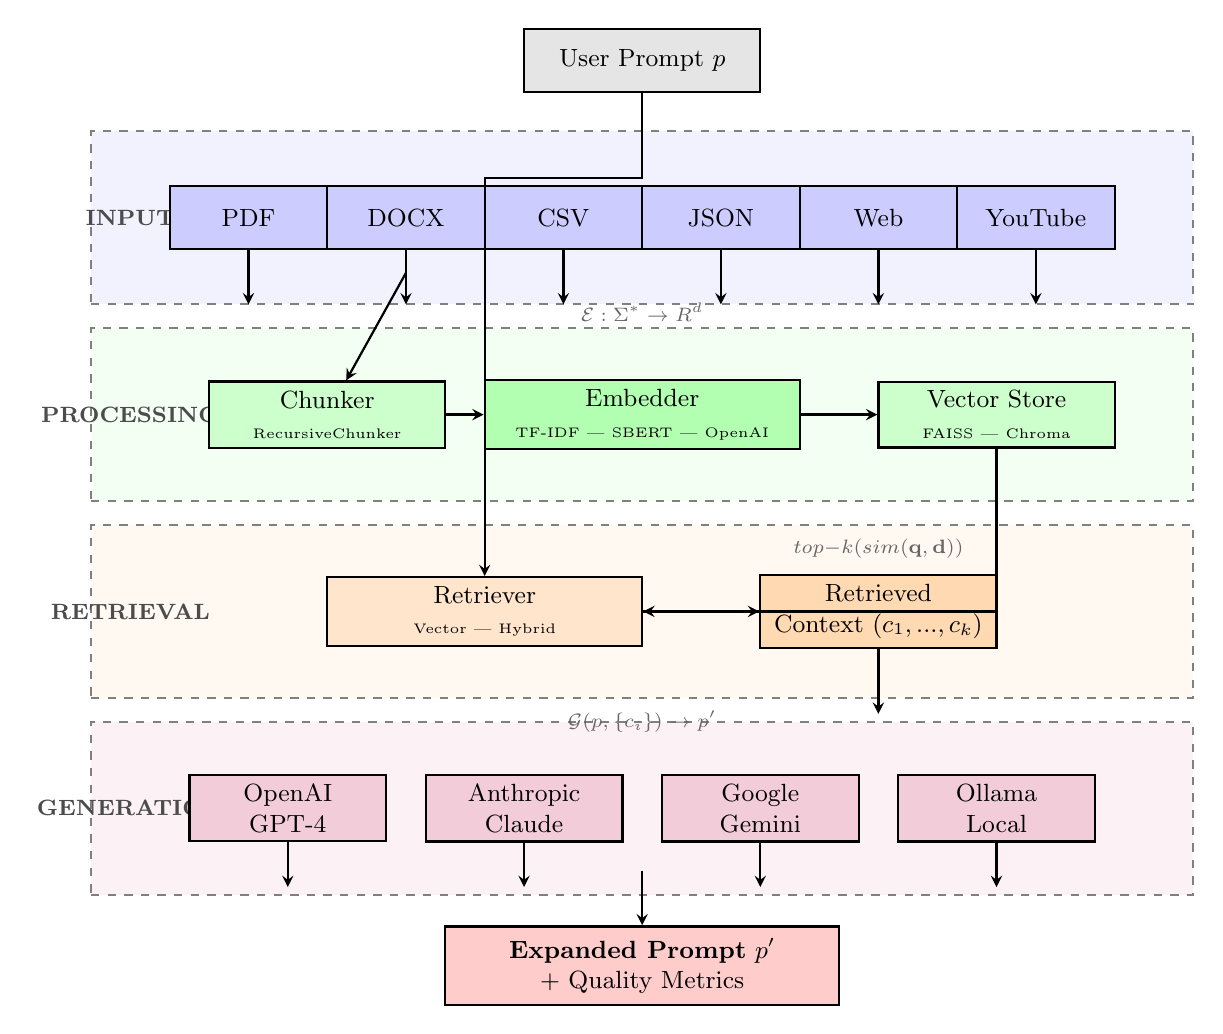
\begin{tikzpicture}[
    node distance=0.8cm and 1.2cm,
    box/.style={rectangle, draw=black, thick, minimum width=2cm, minimum height=0.8cm, align=center, font=\small},
    layer/.style={rectangle, draw=black!50, dashed, thick, minimum width=14cm, minimum height=2.2cm, align=center},
    arrow/.style={->, thick, >=stealth},
    label/.style={font=\footnotesize\bfseries, text=black!70}
]

% Layer backgrounds
\node[layer, fill=blue!5] (input_layer) at (0, 6) {};
\node[layer, fill=green!5] (process_layer) at (0, 3.5) {};
\node[layer, fill=orange!5] (retrieval_layer) at (0, 1) {};
\node[layer, fill=purple!5] (generation_layer) at (0, -1.5) {};

% Layer labels
\node[label] at (-6.5, 6) {INPUT};
\node[label] at (-6.5, 3.5) {PROCESSING};
\node[label] at (-6.5, 1) {RETRIEVAL};
\node[label] at (-6.5, -1.5) {GENERATION};

% Input Layer - Document Loaders
\node[box, fill=blue!20] (pdf) at (-5, 6) {PDF};
\node[box, fill=blue!20] (docx) at (-3, 6) {DOCX};
\node[box, fill=blue!20] (csv) at (-1, 6) {CSV};
\node[box, fill=blue!20] (json) at (1, 6) {JSON};
\node[box, fill=blue!20] (web) at (3, 6) {Web};
\node[box, fill=blue!20] (youtube) at (5, 6) {YouTube};

% Processing Layer
\node[box, fill=green!20, minimum width=3cm] (chunker) at (-4, 3.5) {Chunker\\{\tiny RecursiveChunker}};
\node[box, fill=green!30, minimum width=4cm] (embedder) at (0, 3.5) {Embedder\\{\tiny TF-IDF | SBERT | OpenAI}};
\node[box, fill=green!20, minimum width=3cm] (vectorstore) at (4.5, 3.5) {Vector Store\\{\tiny FAISS | Chroma}};

% Retrieval Layer
\node[box, fill=orange!20, minimum width=4cm] (retriever) at (-2, 1) {Retriever\\{\tiny Vector | Hybrid}};
\node[box, fill=orange!30, minimum width=3cm] (context) at (3, 1) {Retrieved\\Context $(c_1,...,c_k)$};

% Generation Layer
\node[box, fill=purple!20, minimum width=2.5cm] (openai) at (-4.5, -1.5) {OpenAI\\GPT-4};
\node[box, fill=purple!20, minimum width=2.5cm] (anthropic) at (-1.5, -1.5) {Anthropic\\Claude};
\node[box, fill=purple!20, minimum width=2.5cm] (google) at (1.5, -1.5) {Google\\Gemini};
\node[box, fill=purple!20, minimum width=2.5cm] (ollama) at (4.5, -1.5) {Ollama\\Local};

% Output
\node[box, fill=red!20, minimum width=5cm, minimum height=1cm] (output) at (0, -3.5) {\textbf{Expanded Prompt} $p'$\\+ Quality Metrics};

% User Input
\node[box, fill=gray!20, minimum width=3cm] (user) at (0, 8) {User Prompt $p$};

% Arrows - Input flow
\foreach \x in {pdf, docx, csv, json, web, youtube} {
    \draw[arrow] (\x) -- +(0, -1.1);
}

% Arrows - Processing flow
\draw[arrow] (-3, 5.3) -- (chunker);
\draw[arrow] (chunker) -- (embedder);
\draw[arrow] (embedder) -- (vectorstore);

% Arrows - Retrieval flow
\draw[arrow] (user) -- +(0, -1.5) -| (retriever);
\draw[arrow] (vectorstore) |- (retriever);
\draw[arrow] (retriever) -- (context);

% Arrows - Generation flow
\draw[arrow] (context) -- +(0, -1.3);
\foreach \g in {openai, anthropic, google, ollama} {
    \draw[arrow] (\g) -- +(0, -1);
}

% Output arrow
\draw[arrow] (0, -2.3) -- (output);

% Formulas
\node[font=\scriptsize, text=black!60] at (0, 4.8) {$\mathcal{E}: \Sigma^* \rightarrow \mathbb{R}^d$};
\node[font=\scriptsize, text=black!60] at (3, 1.8) {$\text{top-}k(\text{sim}(\mathbf{q}, \mathbf{d}))$};
\node[font=\scriptsize, text=black!60] at (0, -0.4) {$\mathcal{G}(p, \{c_i\}) \rightarrow p'$};

\end{tikzpicture}
\caption{PRIME system architecture showing the five-layer pipeline: Input (document loaders), Processing (chunking and embedding), Storage (vector stores), Retrieval (similarity search), and Generation (LLM-based prompt expansion). Each layer implements pluggable components via abstract interfaces.}
\label{fig:architecture}
\end{figure*}

